\label{DHCP - Dynamic Host Control Protocol}
\chapter{DHCP - Dynamic Host Control Protocol}

In this section we will setup an Ip address for Pc1 and Pc2 by sending Dhcp request Via r1

\section{Configure Dhcp by setting the default router and setting the range of IPs}

First we will need run the commands in Vyos mode by running the following in r1 terminal  \textbf{/bin/su -s /bin/vbash - vyos}

\begin{figure}[H]
\centering
  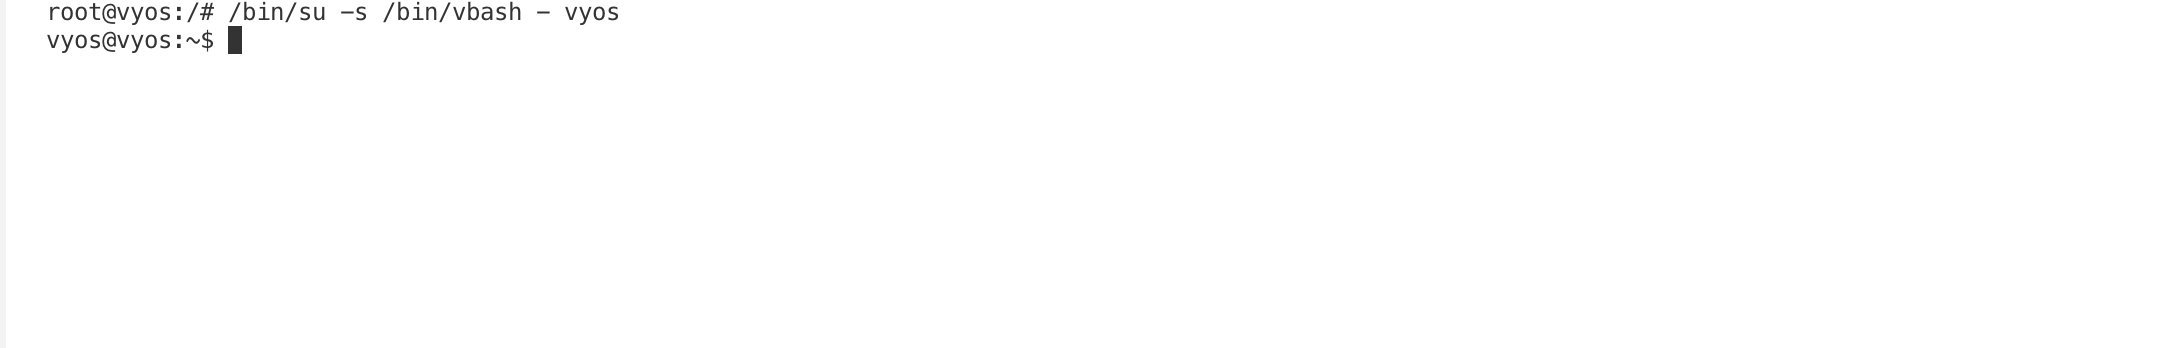
\includegraphics[width=400pt]{Images/vyosmode.png}
  \caption{Set Terminal to be in Vyos mode}
  \label{fig:3.1}
\end{figure}
\section{Dhcp Configuration in r1 and explaining how DHCP is working.}
In order to configure Dhcp and setup ip range and everything  we will need first to run \textbf{Configure} then setup everything for dhcp and after that we run Commit. After running Configure, 
\begin{itemize}
  \item We will enable dhcp-server authoritative for the machine we are running which is r1 in that case
  \item We will setup the default router to be r1 
  \item We will setup the IPs range that can be provided by dhcp server to be from 10.10.0.100/24 to 10.10.0.200/24
\end{itemize}
After setting dhcp we will run commit and that`s it

\begin{figure}[H]
\centering
  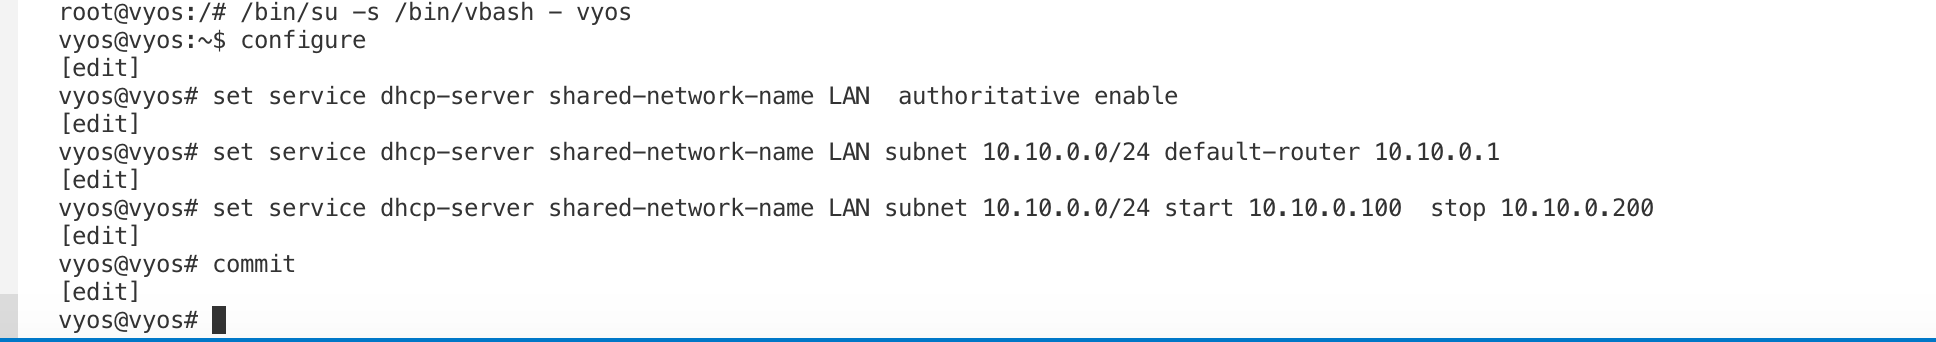
\includegraphics[width=400pt]{Images/dhcpset-up.png}
  \caption{Dhcp configuration in r1}
  \label{fig:3.2}
\end{figure}

\section{Pc1 and Pc2 request ip address from Dhcp server}
Lets see the steps first on Pc1 and same will be for Pc2
\begin{itemize}
  \item pc1 will broadcast that it needs an ip address to all the devices in the same network (Dhcp-Discover).
  \item the default-router (r1) will send request to Dhcp-server. Dhcp gets the message from pc1 it will send Dhcp-offer with ip address \textbf{Note the offered ip will be within the range we provided for dhcp-server} 
  \item if Pc1 accepted the offer it will send Dhcp-Request
  \item Dhcp will get the Request with acceptance and send back Dhcp-Pack which is the acknowledgement along with the ip address, the sub-net mask and the default gateway and the dns-server. Dhcp will keep the record that Pc1 took this ip address

\end{itemize}


\begin{figure}[H]
\centering
  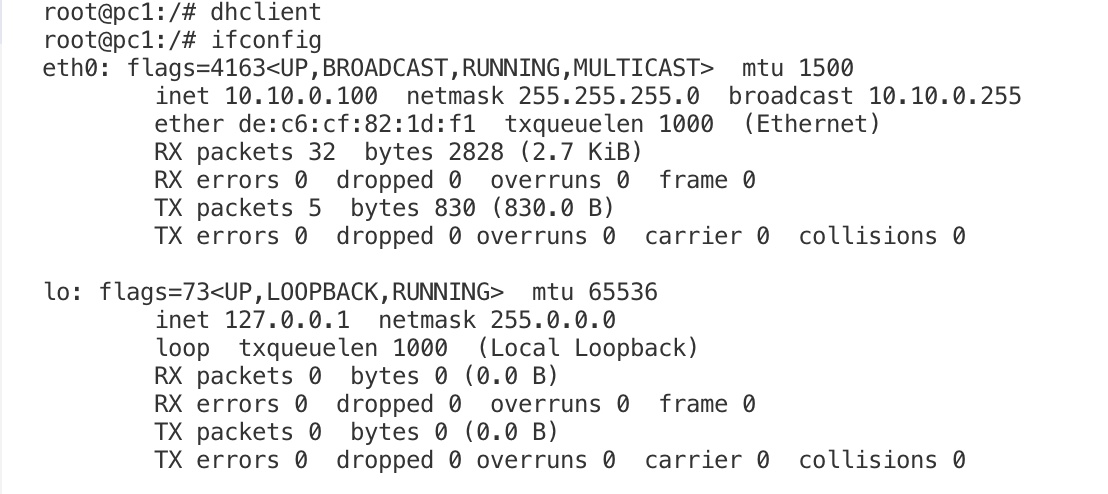
\includegraphics[width=400pt]{Images/pc1DhcpReq.png}
  \caption{Pc1 request for ip}
  \label{fig:3.3}
\end{figure}

\begin{figure}[H]
\centering
  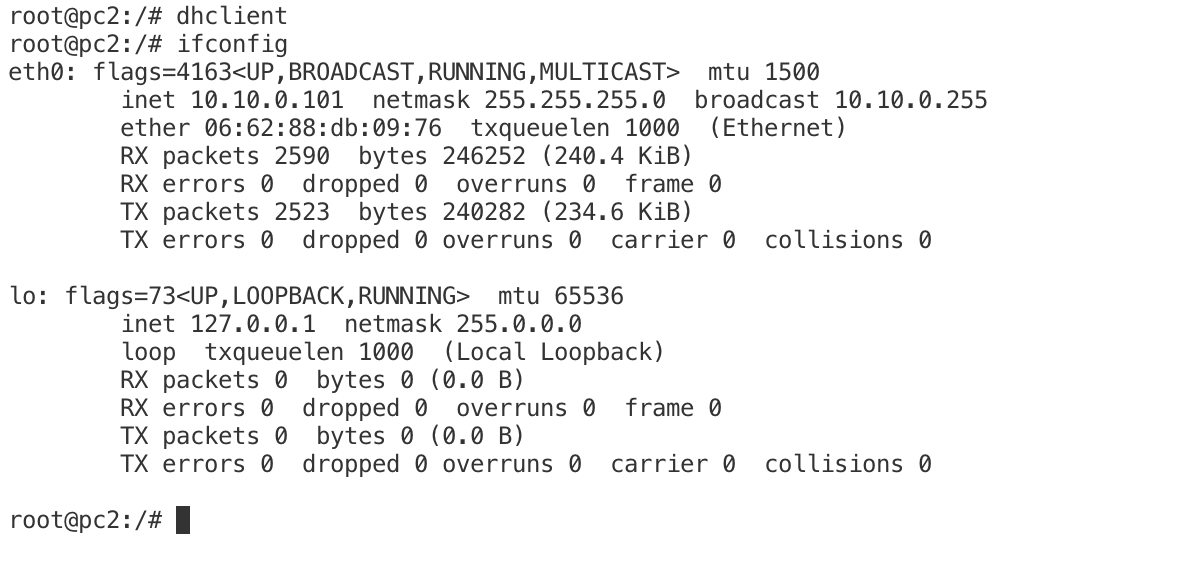
\includegraphics[width=400pt]{Images/pc2DhcpReq.png}
  \caption{Pc2 Request for ip}
  \label{fig:3.4}
\end{figure}


\begin{figure}[H]
\centering
  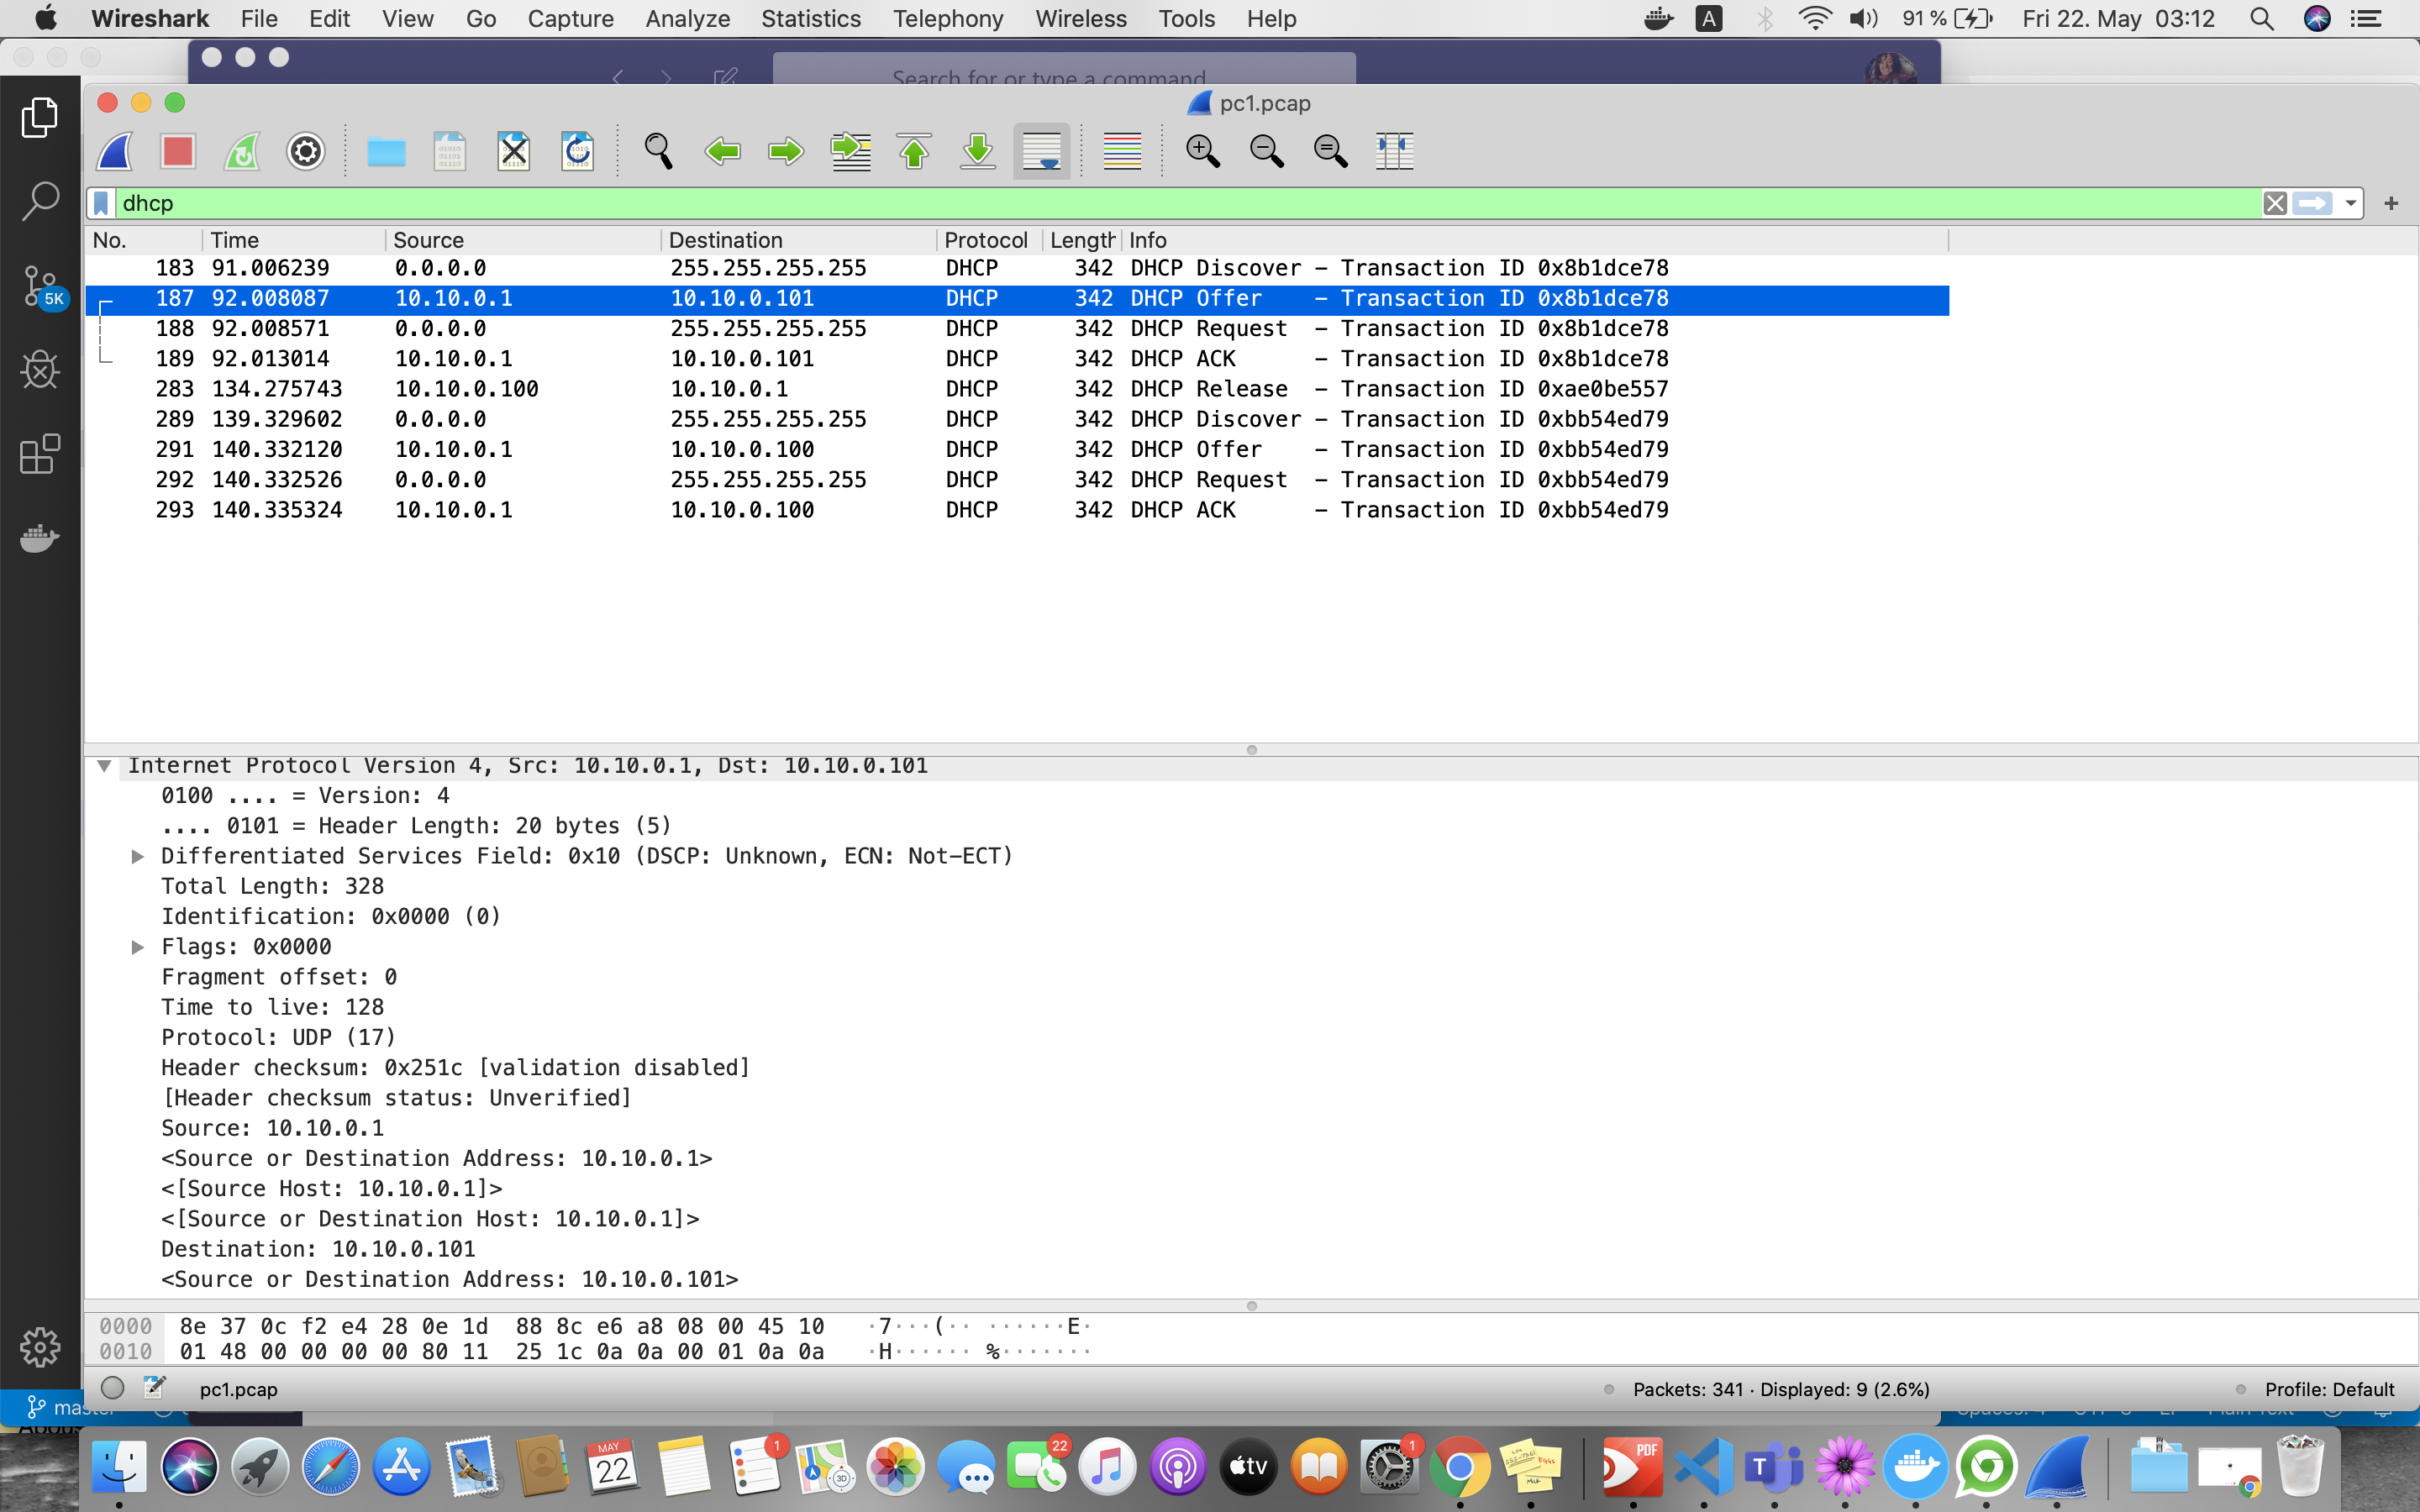
\includegraphics[width=300pt]{Images/dhcpWireshark.png}
  \caption{Pc1 request for ip address procedure as explained represented on wireshark}
  \label{fig:3.5}
\end{figure}

Now lets make sure of the connectivity and that r1 will be connected automatically to pc1 and pc2 by sending ping to Web2 and capture the ICMP request by wire shark


\begin{figure}[H]
\centering
  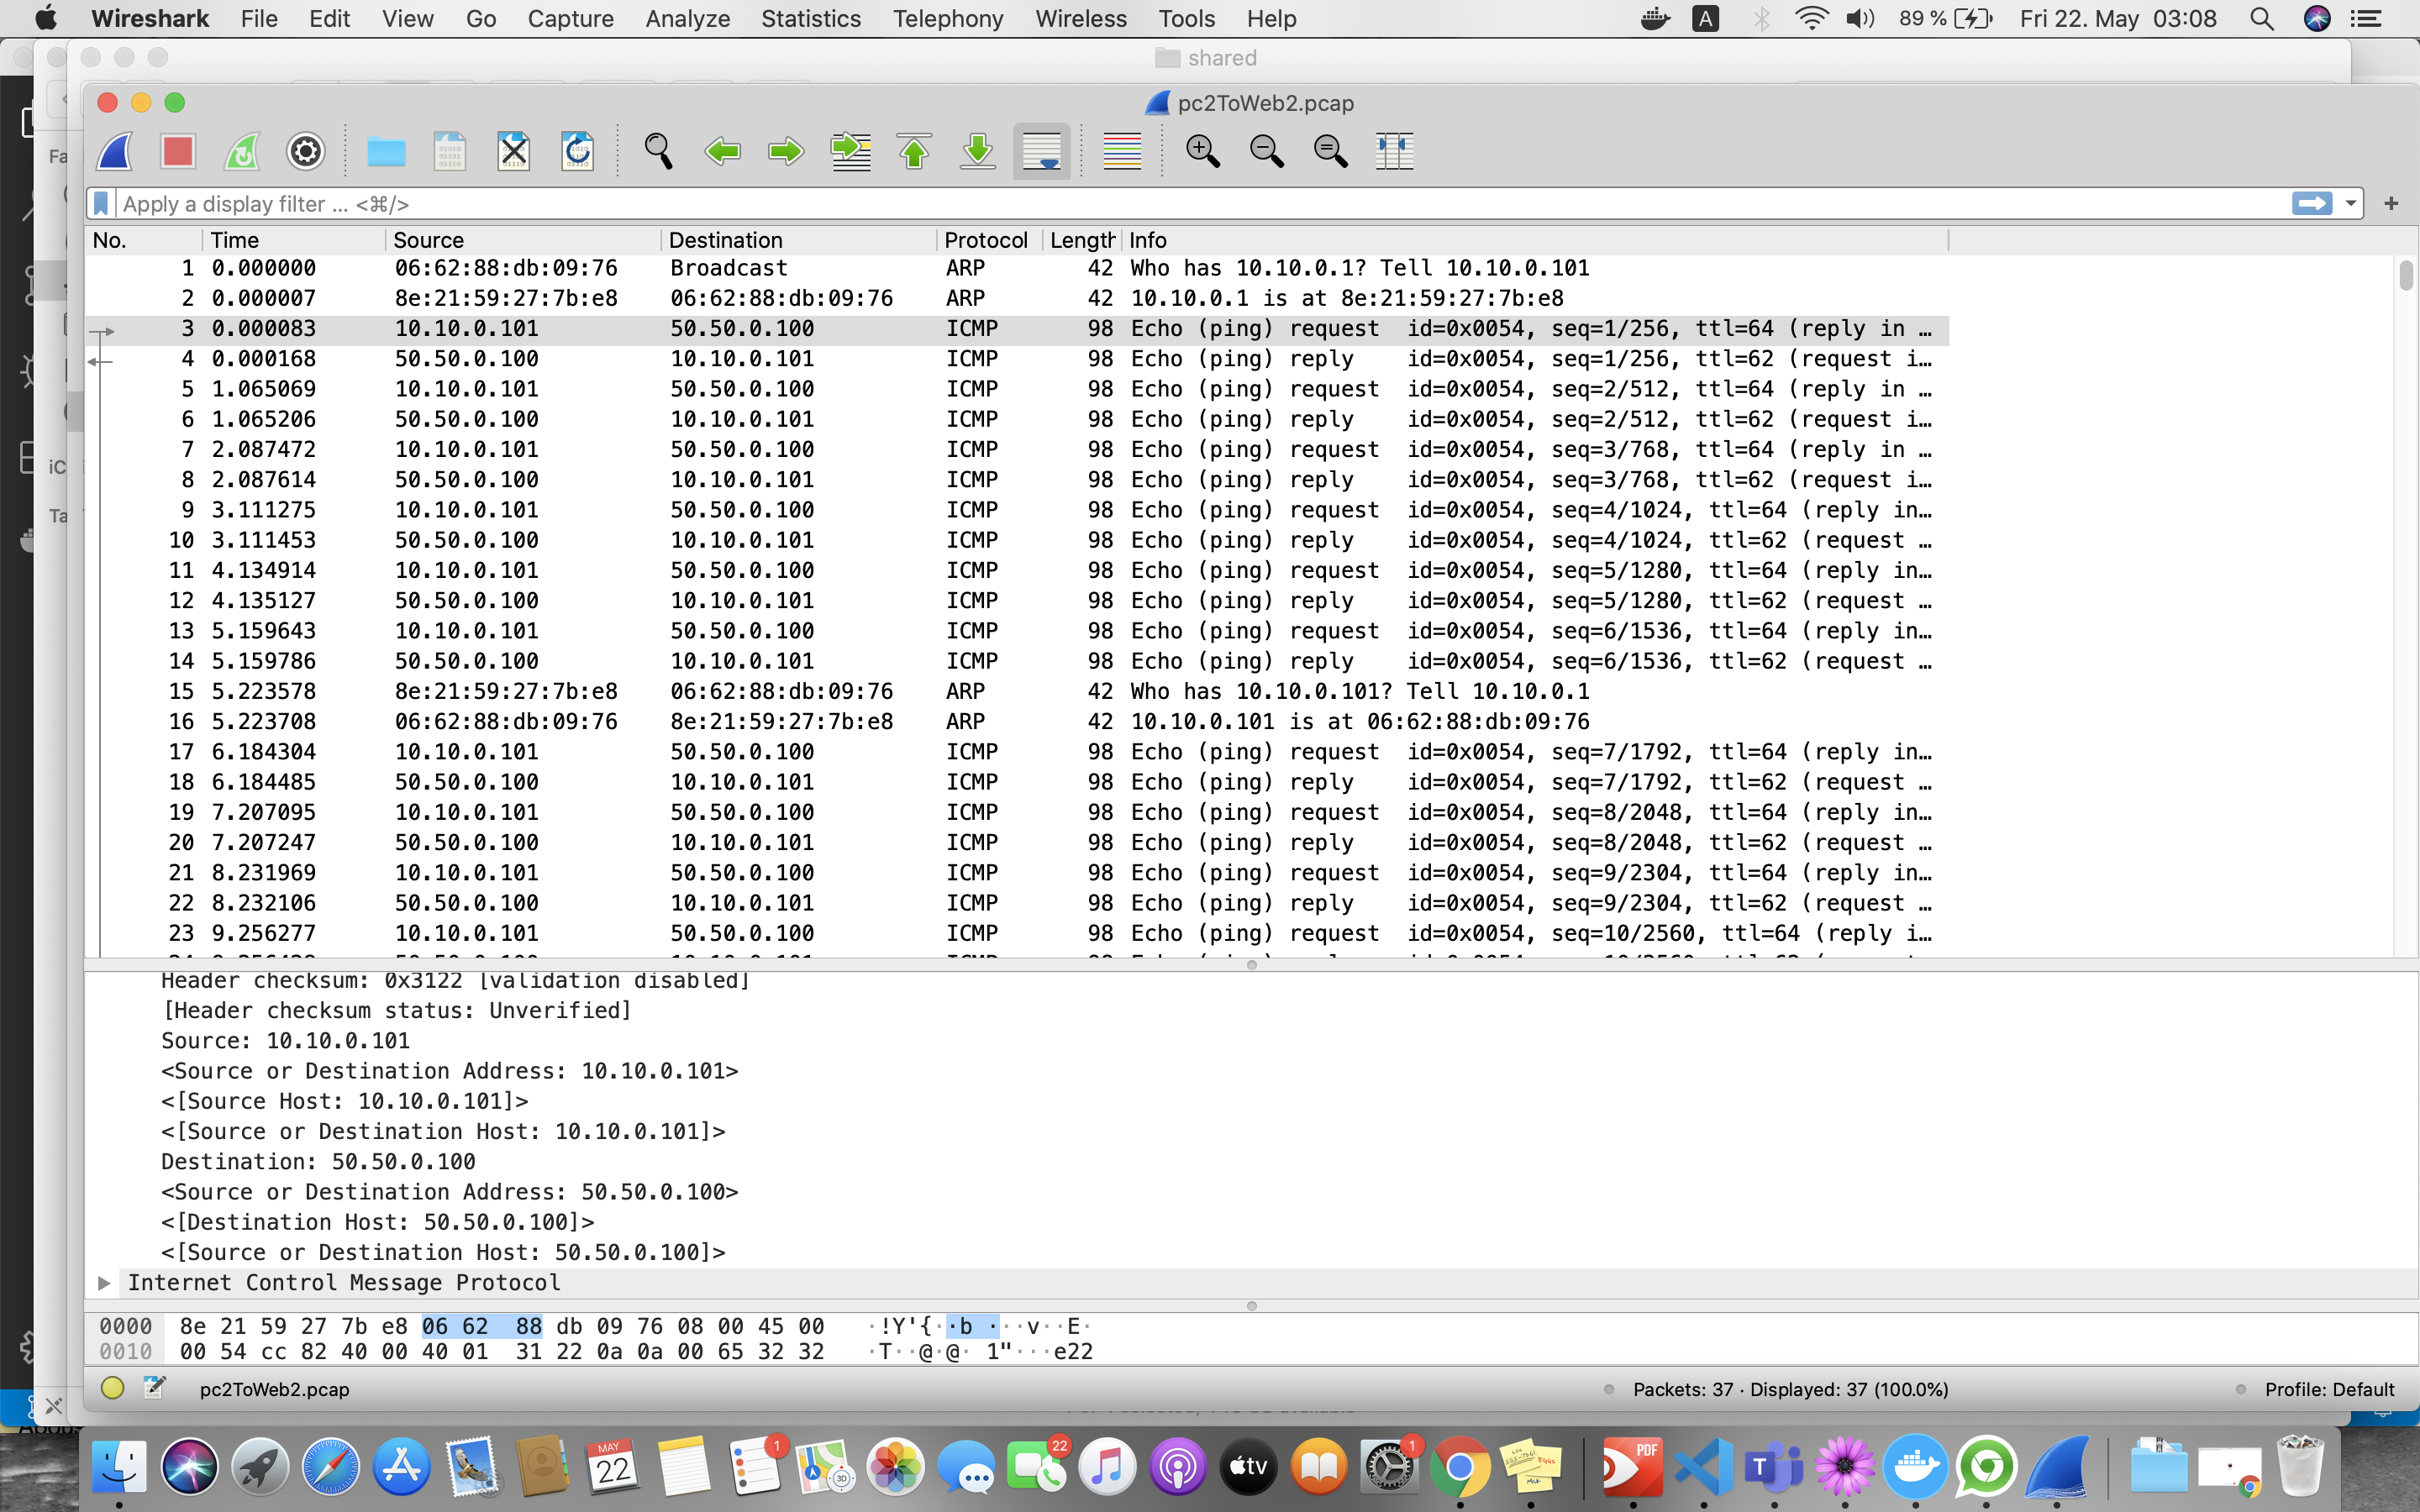
\includegraphics[width=400pt]{Images/pc2Toweb2P3.png}
  \caption{Capturing ICMP on wireshark after pc2 send ping to web2, to ensure connectivity}
  \label{fig:3.7}
\end{figure}